\section{Behavior Inference}\label{sec:infer}

In this section, we introduce a way to infer possible behaviors of a selected
language feature using the \textit{reachability analysis} on the mechanized
specification with the corresponding \textit{syntactic view}.  We first
introduce $\ires$ as the specification language for the mechanized specification
extracted from ECMA-262.  Then, we formally define a syntactic view as an
extension of a JavaScript abstract syntax tree (AST) wtith abstract nodes with
type bounds.  Finally, we formally define the reachability analysis on the
mechanized specialization with a given syntactic view and prove its soundness.

\subsection{$\ires$: Intermediate Representation for ECMAScript Specification}

$\esmeta$ extracts a mechanized specification from ECMA-262 by compiling each
abstract algorithm to the corresponding function of $\ires$, an
\underline{I}ntermediate \underline{R}epresentation for \underline{E}CMAScript
\underline{S}pecification.  Its abstract syntax is defined as follows:

\[
  \begin{array}{lr@{~}c@{~}c@{~}c@{~}l}
    \text{Programs} & \progset &\ni& \prog &=& (\initstset,
    \getfunc, \getinst, \getnext)\\

    \text{Functions} & \funcset &\ni& \func &::=&
    \kwdef \; \kwrl \varx^* \kwrr \; \lab\\

    \text{Instructions} & \instset &\ni& \inst &::=&
    \refer \kweq \expr \mid
    \varx \kweq \kwcl \kwcr \mid
    \varx \kweq \expr \kwrl \expr^* \kwrr \mid \\&&&&&
    \kwif \; \expr \; \lab \; \lab \mid
    \kwret \; \expr\\

    \text{Expressions} & \exprset &\ni& \expr &::=&
    \pval \mid
    \op \kwrl \expr^* \kwrr \mid
    \refer\\

    \text{References} & \referset &\ni& \refer &::=&
    \varx \mid \expr \kwsl \expr \kwsr\\

    \text{Variables} & \varset &\ni& \varx &&

    \text{Labels} \qquad \labset \ni \lab\\
  \end{array}
\]

An $\ires$ program $\prog = (\initstset, \getfunc,
\getinst, \getnext) \in \progset $ consists of initial states
$\initstset$ and three mappings; $\getfunc: \labset \rightarrow
\funcset$ and $\getinst: \labset \rightarrow \instset$ map labels to
their functions and instructions, respectively, and $\getnext: \labset
\rightarrow \labset$ maps labels to their next labels, where a label $\lab \in
\labset$ denotes a program point.  A function $\func \in \funcset$ is defined
with its parameters and body label.  For presentation brevity, we assume that no
global or captured variables exist in this paper.  An instruction $\inst \in
\instset$ is an assignment $\refer \kweq \expr$, an object allocation $\varx
\kweq \kwcl \kwcr$, a function call $\varx \kweq \expr \kwrl \expr^* \kwrr$, a
branch $\kwif \; \expr \; \lab \; \lab$, or a return instruction $\kwret \;
\expr$.  An invocation of an abstract algorithm in ECMA-262 is compiled to a
function call instruction with a new temporary variable.  We represent loops
using branch instructions with cyclic pointing of labels in $\getnext$.
An expression is a primitive value $\pval$, an operation $\op \kwrl \expr^*
\kwrr$, or a reference $\refer$.  A reference is a variable $\varx$ or an object
field $\expr \kwsl \expr \kwsr$.  We write $\expr.\varf$ to briefly represent
$\expr \kwsl \code{"f"} \kwsr$.

We define the concrete semantics $\sem{\prog}$ of an $\ires$ program $\prog$ as
a set of reachable state from the initial states $\initstset$ of the
program:
\[
  \sem{\prog} = \{ \st \in \stset \mid \exists \initst \in \initstset. \;
  \initst \trans^* \st \}
\]
where $\trans^*$ denotes one or more repetition of $\trans$, and
$\st \trans \st'$ if and only if $\st = (\lab, \_, \_, \_)$ and
$\sem{\getinst(\lab)}(\st) = \st'$.  We also define the denotational
semantics of expressions $\sem{\expr}: \stset \rightarrow \valset$ and
instructions $\sem{\inst}: \stset \rightarrow \stset$ where $\stset$ and
$\valset$ denote states and values, respectively.  However, for
brevity, we omit them in this paper and refer the interested readers to a
companion report~\cite{report}.  Another way to represent the concrete semantics
is to define a transfer function $\transfer: \powerset{\stset} \rightarrow
\powerset{\stset}$:
\[
  \sem{\prog} = \lim_{n \rightarrow \infty}\transfer^n(\initstset)
\]
where
\begin{equation}\label{eqn:transfer}
  \transfer(S) =
  \{ \st' \in \stset \mid \exists \st \in S. \; \st \trans \st' \}
\end{equation}

In $\ires$, JavaScript ASTs are values as well, and they are defined with tree
nodes $\nodeset$ as follows:
\[
  \begin{array}{l@{~}c@{~}l@{~}c@{~}l}
    \treeset &\ni& \tree &::=& \nt_k \langle \node^* \rangle\\
    \nodeset &\ni& \node &::=& \str \mid \tree\\
  \end{array}
\]
A JavaScript AST $\nt_k \langle \node_1, \cdots, \node_n \rangle$ denotes $k$-th
alternative in the syntactic production of nonterminal symbol $\nt$ with
multiple tree nodes $\node_1, \cdots, \node_n$.  A tree node is a string $\str$
for a terminal symbol or another tree $\tree$ for a nonterminal symbol. We
define several notations to easily deal with JavaScript ASTs.  The notation
$\nt_k.\eval$ denotes an \esalg{Evaluation} function of $k$-th alternative in
the production of $\nt$.  Similarly, the notation $\tree.\eval$ denotes the
\esalg{Evaluation} function of the AST $\tree$, and it is same with
$\nt_k.\eval$ when $\tree = \nt_k \langle \cdots \rangle$. The
\esalg{Evaluation} of each AST takes the AST itself and its tree nodes that are
nonterminals as arguments.  The notation $\getsubs(\tree)$ denotes tree nodes
that are subtrees of $\tree$.

For example, Figure~\ref{fig:add-eval} (a) shows a syntactic production for
additive expressions.  Consider a JavaScript expression: \jscode{1 + 2}.  Then,
the following AST is produced as its parsing result:
\[
  \begin{array}{lcl}
    \tree_0 &=&
    \essyn{AdditiveExpression}_1 \langle \tree_1, \code{"+"}, \tree_2 \rangle\\

    \tree_1 &=&
    \essyn{AdditiveExpression}_0 \langle \cdots \rangle\\

    \tree_2 &=&
    \essyn{MultiplicativeExpression}_0 \langle \cdots \rangle\\
  \end{array}
\]
\begin{figure}[H]
  \vspace*{-1em}
  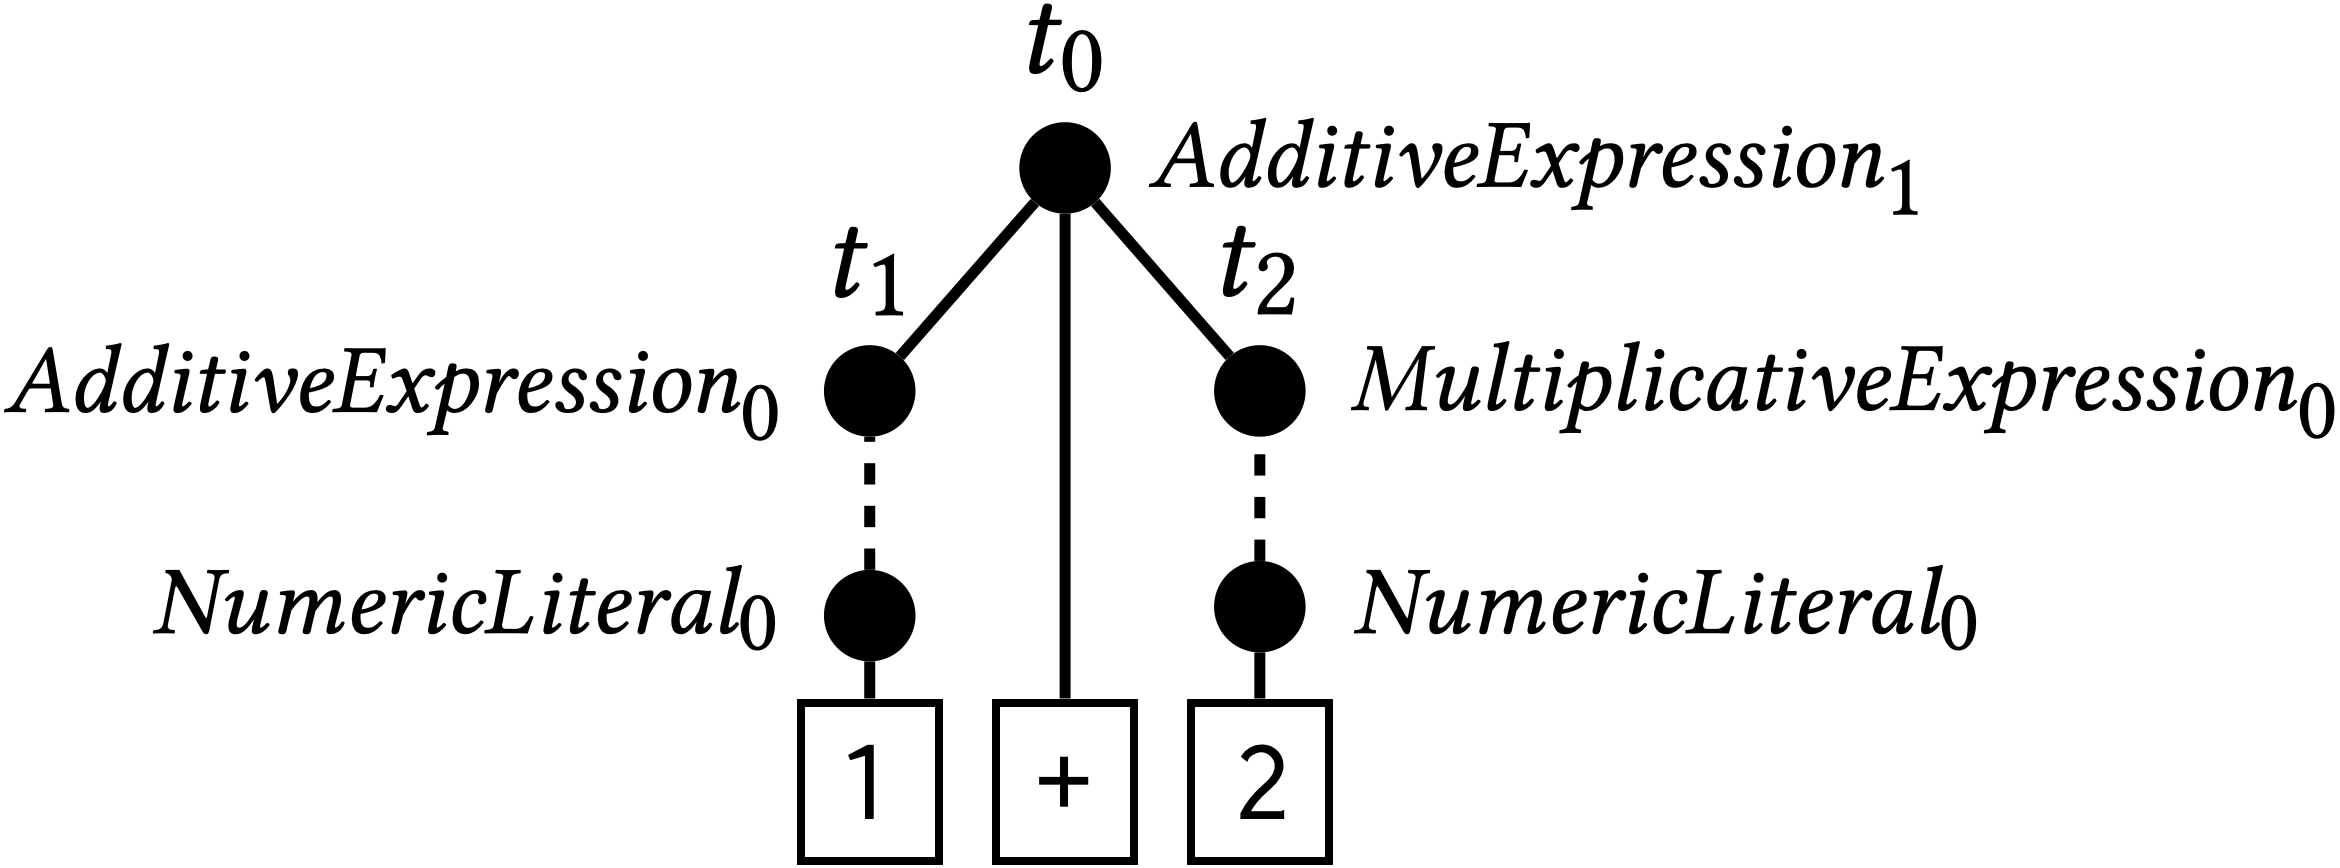
\includegraphics[width=.7\columnwidth]{img/add-ast.png}
  \vspace*{-1em}
\end{figure}
\noindent Its \esalg{Evaluation} function $\essyn{AdditiveExpression}_1.\eval$
takes three subtrees as arguments annotated by $\tree_0$, $\tree_1$, and
$\tree_2$ in the figure. They are subtrees of $\tree_0$ (i.e., $\tree_0 \subtree
\tree_0, \cdots, \tree_3 \subtree \tree_0$), and $\getsubs(\tree_0) = [\tree_1,
\tree_2]$.

\subsection{Syntactic Views}\label{sec:view}

We introduce a \textit{syntactic view} $\atree \in \atreeset$ as an extended
JavaScript AST defined with abstract tree nodes $\anodeset$ with type bounds:
\[
  \begin{array}{l@{~}c@{~}l@{~}c@{~}l}
    \atreeset &\ni& \atree &::=& \nt_k \langle \anode^* \rangle \mid \nt: \ty \\
    \anodeset &\ni& \anode &::=& \str \mid \atree\\
  \end{array}
\]
where $\nt: \ty$ denotes an abstract node whose nonterminal symbol is $\nt$ and
evaluation result has a type $\ty$.  We define the concretization of abstract
trees $\atreegamma: \atreeset \rightarrow \powerset{\treeset}$ and that of
abstract nodes $\anodegamma: \anodeset \rightarrow \powerset{\nodeset}$ as
follows:
\[
  \begin{array}{lcl}
    \atreegamma(\nt_k \langle \anode_1, \cdots, \anode_n \rangle) &=&
    \{ \nt_k \langle \node_1, \cdots, \node_n \rangle \mid \node_j \in
    \anodegamma(\anode_j) \}\\

    \atreegamma(\nt) &=&
    \{ \tree \in \treeset \mid \tree = \nt_k \langle \cdots \rangle \}\\

    \anodegamma(\str) &=& \{ \str \}\\

    \anodegamma(\atree) &=& \atreegamma(\atree)\\
  \end{array}
\]

% \[
%   \begin{array}{lcl}
%     \anode \order \anode' &\Leftrightarrow& \left\{
%       \begin{array}{ll}
%         \anode = \anode' &\vee\\
% 
%         \anode' = \nt &\vee\\
% 
%         (\anode = \atree \wedge \anode' = \atree' \wedge \atree \order
%         \atree')\\
%       \end{array}
%     \right.\\
% 
%     \atree \order \atree' &\Leftrightarrow& \left\{
%       \begin{array}{ll}
%         \atree = \atree' &\vee\\
% 
%         \atree' = \treetop &\vee\\
% 
%         \begin{array}{@{}l@{}}
%           \atree = \nt_k \langle \atree_1, \cdots, \atree_n \rangle \wedge
%           \atree' = \nt_k \langle \atree'_1, \cdots, \atree'_n \rangle \wedge\\
%           \forall j. \; \tree_j \order \tree'_j\\
%         \end{array}\\
%       \end{array}
%     \right.\\
% 
%     \atree \join \atree' &=& \left\{
%       \begin{array}{ll}
%         \atree' & \text{if} \; \atree \order \atree'\\
% 
%         \atree & \text{if} \; \atree \revorder \atree'\\
% 
%         \nt_k \langle \atree''_1, \cdots, \atree''_n \rangle &
%         \text{if} \; \atree = \nt_k \langle \atree_1, \cdots, \atree_n \rangle
%         \wedge\\&
%         \phantom{\text{if} \;} \atree = \nt_k \langle \atree_1, \cdots, \atree_n
%         \rangle \wedge\\&
%         \phantom{\text{if} \;} \forall j. \; \atree''_j = \atree_j
%         \join \atree'_j\\
%         \treetop & \text{otherwise}\\
%       \end{array}
%     \right.\\
%   \end{array}
% \]
We define
In addition, we define abstract subtree relation $\asubtree \subseteq \atreeset
\times \treeset$:
\[
  \atree \; \asubtree \; \tree' \iff \exists \tree \in \atreegamma(\atree). \;
  \tree \subtree \tree'
\]
to filter out JavaScript programs not related to a given syntactic view.
Similar to $\getsubs(\tree)$, an abstract helper function $\agetsubs(\atree)$
denotes abstract tree nodes that are syntactic views when $\atree = \nt_k
\langle \cdots \rangle$.

\subsection{Reachability Analysis}\label{sec:view}

\todo
